\documentclass{beamer}
% Some basic packages
\usepackage[utf8]{inputenc}
\usepackage[T1]{fontenc}
\usepackage{textcomp}
\usepackage[english]{babel}
\usepackage{url}
\usepackage{graphicx}
\usepackage{float}
\usepackage{booktabs}
\usepackage{listings}
\usepackage{dcolumn}
\newcolumntype{2}{D{.}{}{2.0}}
\usepackage{xcolor}

\definecolor{codegreen}{rgb}{0,0.6,0}
\definecolor{codegray}{rgb}{0.5,0.5,0.5}
\definecolor{codepurple}{rgb}{0.58,0,0.82}
\definecolor{backcolour}{rgb}{0.95,0.95,0.92}

\lstdefinestyle{mystyle}{
    backgroundcolor=\color{backcolour},   
    commentstyle=\color{codegreen},
    keywordstyle=\color{magenta},
    numberstyle=\tiny\color{codegray},
    stringstyle=\color{codepurple},
    basicstyle=\ttfamily\footnotesize,
    breakatwhitespace=false,         
    breaklines=true,                 
    captionpos=b,                    
    keepspaces=true,                 
    numbers=left,                    
    numbersep=5pt,                  
    showspaces=false,                
    showstringspaces=false,
    showtabs=false,                  
    tabsize=2
}

\lstset{style=mystyle}

%\pdfminorversion=7

\usepackage[
    backend=biber,
    style=authoryear-icomp,
    sortlocale=auto,
    natbib=true,
    url=false, 
    doi=true,
    eprint=false
]{biblatex}
% \addbibresource{example.bib}

\usepackage{hyperref}
\hypersetup{
	colorlinks=true,
}


\addbibresource{zotero.bib}
% Figure support as explained in my blog post.
\usepackage{import}
\usepackage{xifthen}
\usepackage{pdfpages}
\usepackage{transparent}
\newcommand{\incfig}[1]{%


    \def\svgwidth{\columnwidth}
    \import{./figures/}{#1.pdf_tex}
}

\title{Limiting Distributions of Self-Interacting Random Walks}
\author{Xiaoyu Liu, Lei Fu. Supervisor: Prof. Jonathon Peterson, Julia Garner}

\usetheme{purdue}

\begin{document}
\begin{frame}
	\titlepage
\end{frame}
\begin{frame}
	\frametitle{Outline}
	\tableofcontents
\end{frame}

\section{Motivation and Background}

\begin{frame}
 \frametitle{Simple Random Walk}

 \begin{definition}
 A 1-d simple symmetric random walk (SSRW) is a discrete random process $(X_t)_{t \in \mathbb{N}}$ on $\mathbb{Z}$ where 
 \begin{itemize}
 	\item $X_0 = 0$
	\item $X_t = X_{t-1} + 1$ or $X_{t-1}-1$ with probability $\frac{1}{2}$
 \end{itemize}
 \end{definition}
\pause

By functional central limit theorem, the SSRW converges to a Brownian Motion under proper scaling. In particular the scaled distribution of position at time $t$ converges to normal distribution:
 \[
	 \frac{X_t}{\sqrt{t} } \xrightarrow{d} \mathcal{N}(0,1)
 .\] 


\end{frame}

\begin{frame}
	\frametitle{Simple Random Walk}

	\begin{figure}[htpb]
		\centering
		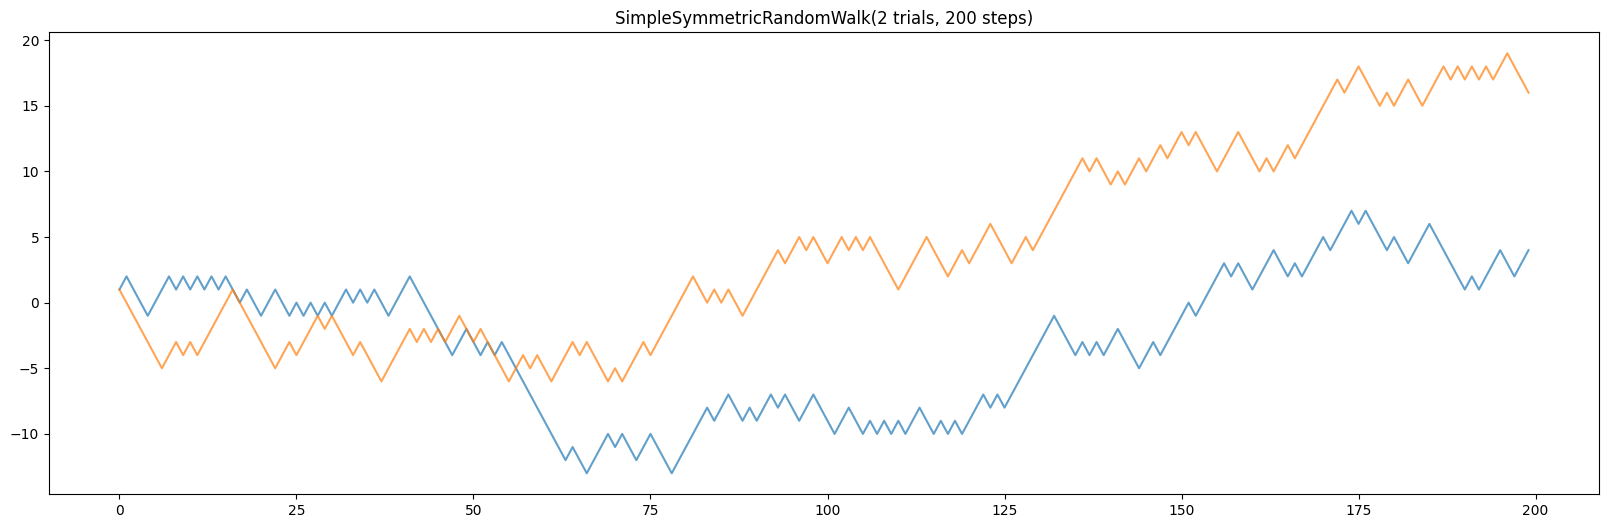
\includegraphics[width=0.8\textwidth]{figures/ssrw-2-200.png}
		%\caption{figure/ssrw-2-200.png}
		%\label{fig:figure-ssrw-2-200-png}
	\end{figure}
	\pause
	\begin{figure}[htpb]
		\centering
		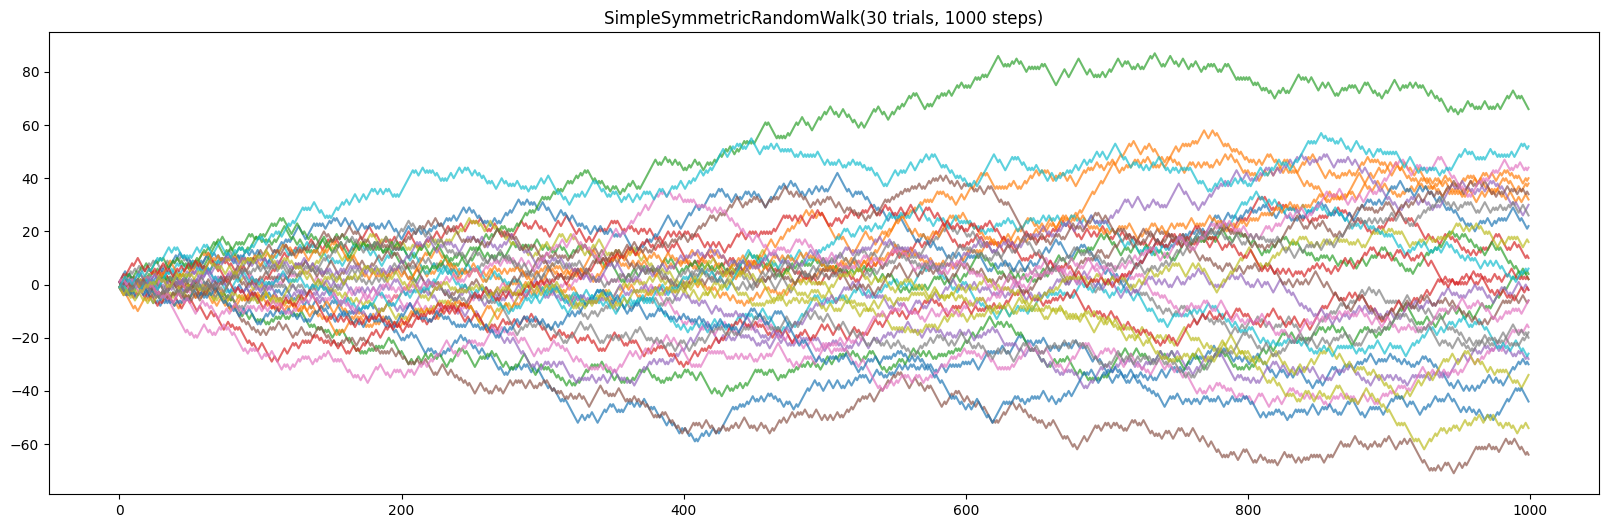
\includegraphics[width=0.8\textwidth]{figures/ssrw-30-1000.png}
	\end{figure}
\end{frame}
\begin{frame}
	\frametitle{Simple Random Walk}
	\begin{figure}[htpb]
		\centering
		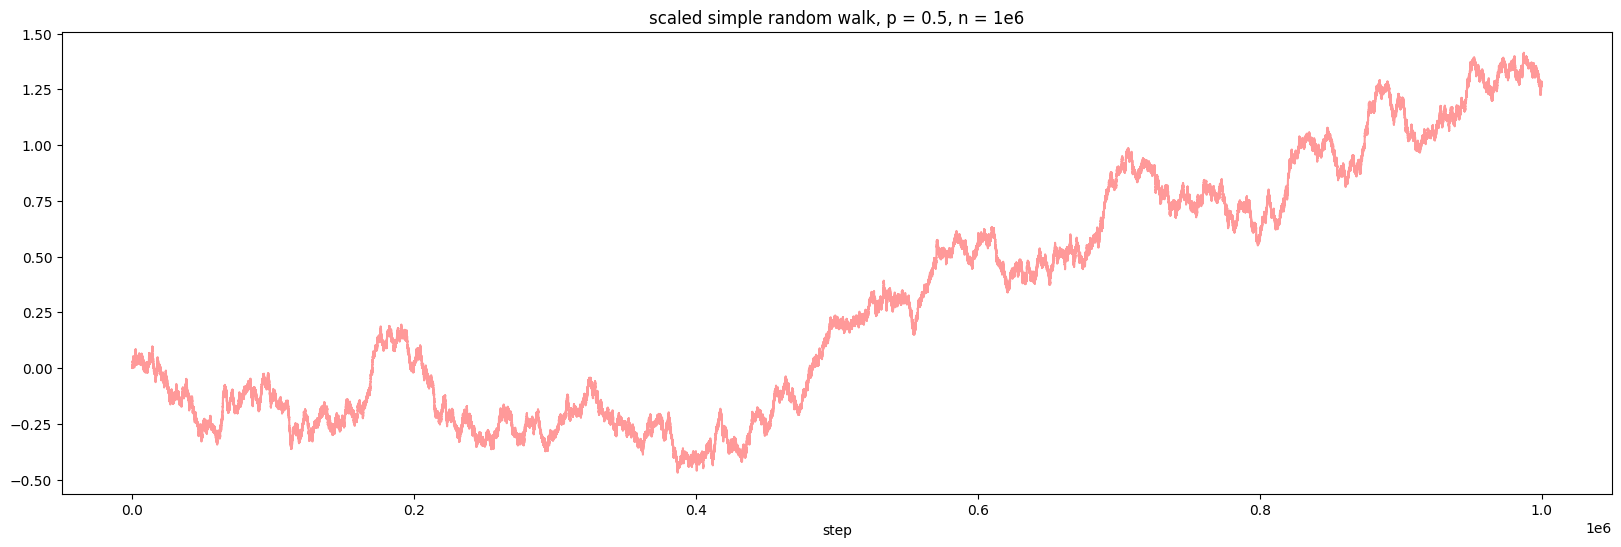
\includegraphics[width=0.8\textwidth]{figures/ssrw-1-1e6-scaled.png}
	\end{figure}
	\pause
	One can prove that scaled limit of the SSRW gives rise to a continuous-time process, which is exactly the Brownian Motion.
\end{frame}

\begin{frame}
	\frametitle{Self-Interacting Random Walk (SIRW)}

	\begin{itemize}
		\item What are the limiting behaviors of more general Random Walks?
	
		\item<2->
	We consider a special type of SIRW, where the tendency to go left or right depends on the number of times that edge has been visited before.

\begin{figure}[ht]
    \centering
    \incfig{sirw-decision}
    \caption{sirw-decision}
    \label{fig:sirw-decision}
\end{figure}
	\end{itemize}
\end{frame}

\begin{frame}
	\frametitle{Self-Interacting Random Walk (SIRW)}
	\begin{definition}
		An SIRW is a discrete random walk on $\mathbb{Z}$ such that for all $t > 0$,
		\begin{multline*}
			\operatorname{Pr} \left[ X_{t} = X_{t - 1} \pm 1 | X_{t-1} =  x_{t-1}, \ldots, X_0 = x_0 \right] =\\
			\frac{W_{t-1}(x_{t-1} \pm 1)}{W_{t-1}(x_{t-1}-1)+W_{t-1}(x_{t-1}+1)}
		.\end{multline*} 
		where 
		\begin{itemize}
			\item $W_{t-1} = w \circ N_{t-1}$
			\item $N_{t}(x) = \sum_{\tau=0}^{t} \mathbf{1}(X_\tau = x)$ counts the number of visits
			\item $w: \mathbb{N} \to \mathbb{R}^+$ is called the \textbf{weight function}, it is required to be monotone, and satisfies some regularity conditions.
		\end{itemize}
	\end{definition}
	
\end{frame}

\begin{frame}
	\frametitle{Examples of SIRWs}

	$w(n) = 1+ \frac{5}{(n+1)^2} = 1+\frac{c}{n}+O\left(n^{-2}\right)$

	The \textbf{Asymptotically Free} case

	\begin{figure}[htpb]
		\centering
		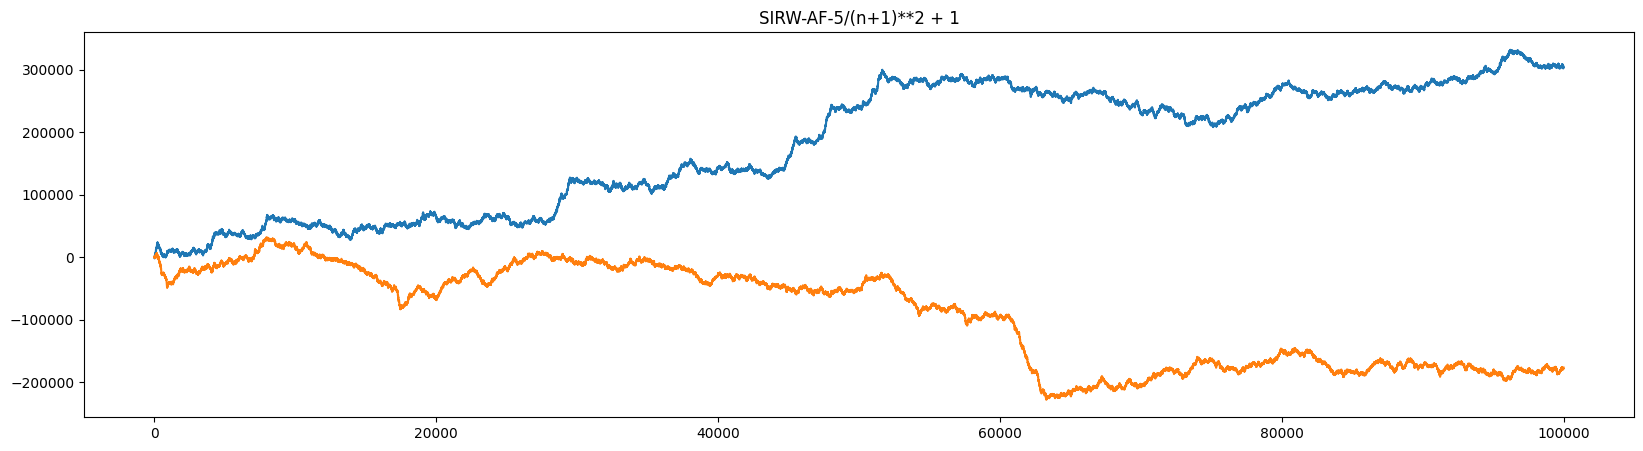
\includegraphics[width=0.8\textwidth]{figures/sirw-af-example.png}
	\end{figure}
	More (or less) ``explorative'',  behaves like SSRW between its extrema.

\end{frame}
\begin{frame}
	\frametitle{Examples of SIRWs}

	$w(n) = \frac{1}{n+1} = n^{- \alpha} + c n^{-1 - \alpha} + O(n^{-2 - \alpha})$

	The \textbf{Polynomially Self-Repelling} case

	\begin{figure}[htpb]
		\centering
		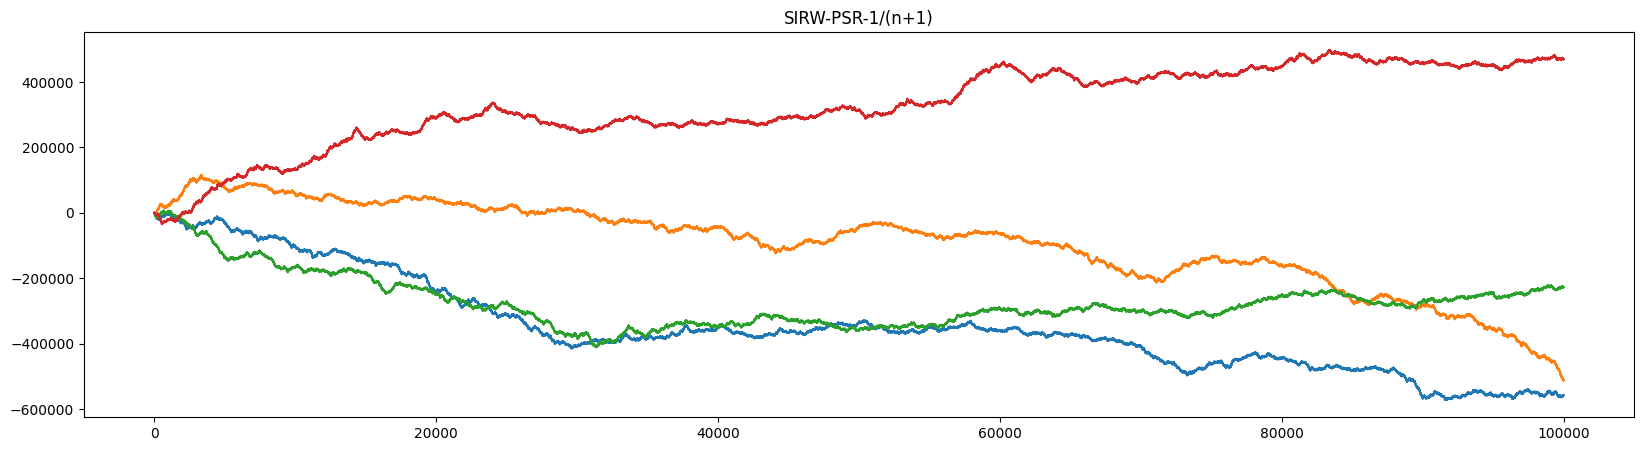
\includegraphics[width=0.8\textwidth]{figures/sirw-psr-example.png}
	\end{figure}
	Does not like to come back to origin!

\end{frame}

\begin{frame}
	\frametitle{Convergence Results for SIRWs}

	How do those SIRWs behave under scaled limit?
\pause
	By \cite{kosyginaConvergenceNonconvergenceScaled2022}, we know that \textbf{Asymptotically Free} SIRWs do have scaled limit:
	\[
		\frac{X_t}{\sqrt{t} } \implies \text{BMPE}(\gamma, \gamma)
	\] 
\pause
	where $\text{BMPE}(\alpha, \beta)$, $\alpha, \beta < 1$ is the Brownian Motion Perturbed at its Extrema:
	\[
		Y_t = B_t + \alpha \sup_{s < t} Y_s + \beta \inf _{s < t} Y_s
	.\] 
\pause
	The parameter $\gamma$ depends on weight function:
	\[
		\gamma(w) = \lim_{n \to \infty} \sum_{k = 0}^{n-1} \frac{1}{w(2 k + 1)} - \frac{1}{w(2 k)}
	.\] 
\end{frame}

\begin{frame}
	
	\begin{figure}[htpb]
		\centering
		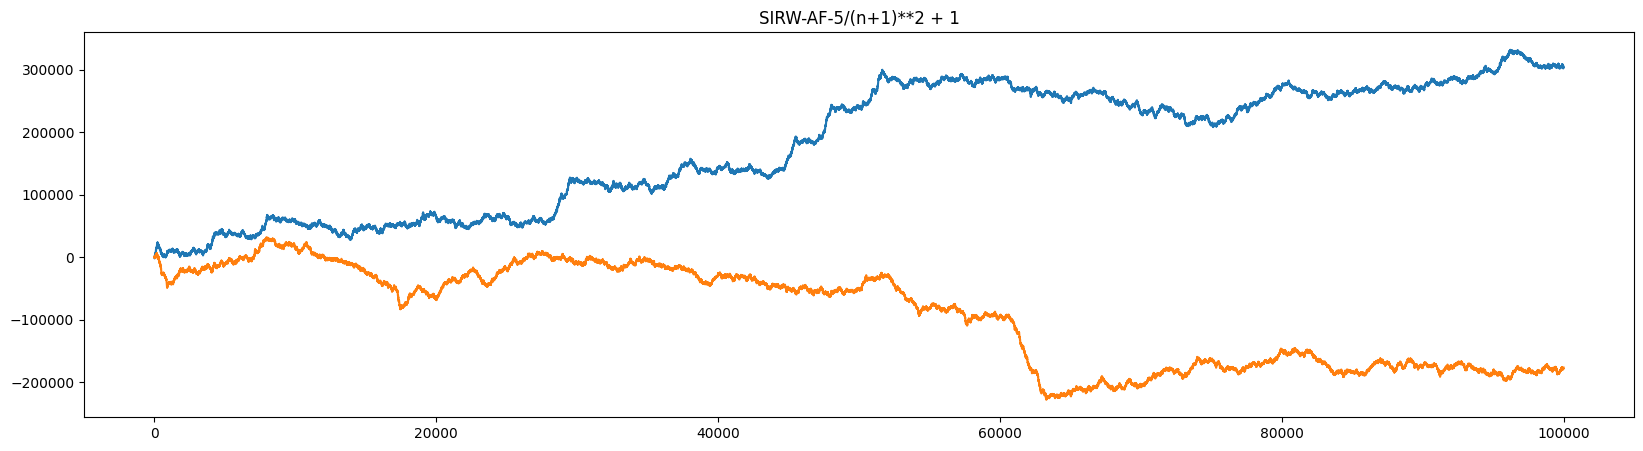
\includegraphics[width=0.8\textwidth]{figures/sirw-af-example.png}
		\caption{Asymptotically Free SIRW with $w(n) > 1$}
	\end{figure}

	\begin{figure}[htpb]
		\centering
		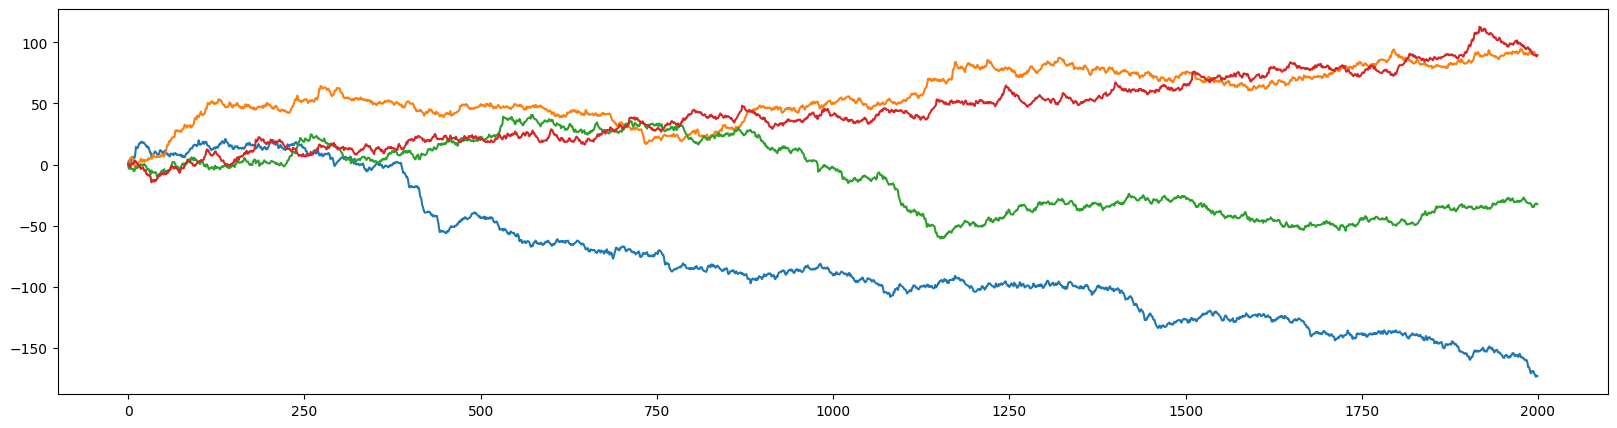
\includegraphics[width=0.8\textwidth]{figures/bmpe-example.png}
		\caption{BMPE with $\gamma(w) > 1$}
	\end{figure}

	
	
\end{frame}

\begin{frame}
	\frametitle{Goal of our study}
	\begin{itemize}
		\item 
	What about the \textbf{Polynomially Self-Repelling} case? {\color{red}\textbf{We don't know.}}
\item<2->
	\cite{tothGeneralizedRayKnightTheory1996} derives an analytic form of the limiting distribution provided the limit exists, but we don't know if the limit exists.
\item <3->
	The goal is to work towards answering this question.
\item <3->
	I will introduce statistical techniques we developed to help answering the question, and some intermediate results.
	\end{itemize}




\end{frame}

\section{Statistical Test of Convergence}
\subsection*{Adapted KS Test}

\begin{frame}
	\frametitle{Statistical test for limiting distribution}

	\begin{itemize}
		\item Let $F_0$ be the postulated limiting distribution of  $X_t$.
		\item At each time $t = m$, we have the distribution $F_m$.
		\item<2-> Take $n$ samples, we have empirical distribution $S_{m, n}$, which can be made continuous by linearization.
		\item<3-> The Kolmogorov-Smirnov Theorem says that $\|S_{m, n} - F_m\|_{\infty } \to  0$ as $m \to  \infty $, and controls the rate of convergence by probabilistic bound.
		\item<4-> If we assume some rate of of convergence of $\|F_m - F_0\|_{\infty }\to 0$, we will be able to control how fast the \textbf{Adapted K-S Statistic} will vanish under \textbf{null hypothesis} $(H_0: F_m \implies F_0)$:
			\[
				D_{m,n} = \|S_{m, n}- F_0\|_{\infty } \to  0
			.\] 
	\end{itemize}
\end{frame}

\begin{frame}
	\frametitle{One-sample Adapted K-S Test}

	\begin{definition}
		We define the one-sample adapted K-S test as follows:
		\begin{itemize}
			\item Null hypothesis $H_0$ : $F_m \implies F_0$ at rate of $m^{-\frac{1}{2}}$ (Similar to Berry-Esseen Theorem)
			\item Test Statistic $D_{m,n}$ is adjusted K-S statistic.
			\item Rejection Criterion:
				\[
				D_{m, n}>\frac{v^*}{\sqrt{n}}=\frac{L^{-1}(1-\alpha)}{\sqrt{n}}+C \sqrt{\frac{1}{m}}
			.\]
			where $L$ is K-S distribution, $C$ is the constant bound for independent increments (which only serves as an approximation).
		\end{itemize}
	\end{definition}
	To run the test, compute $p$-value for a broad range of $m $ and $n$. Reject $H_0$ if the test consistently rejects for all large $m, n$.
\end{frame}

\begin{frame}
	\frametitle{Results of Adapted KS Test}
	\begin{figure}[htpb]
		\centering
		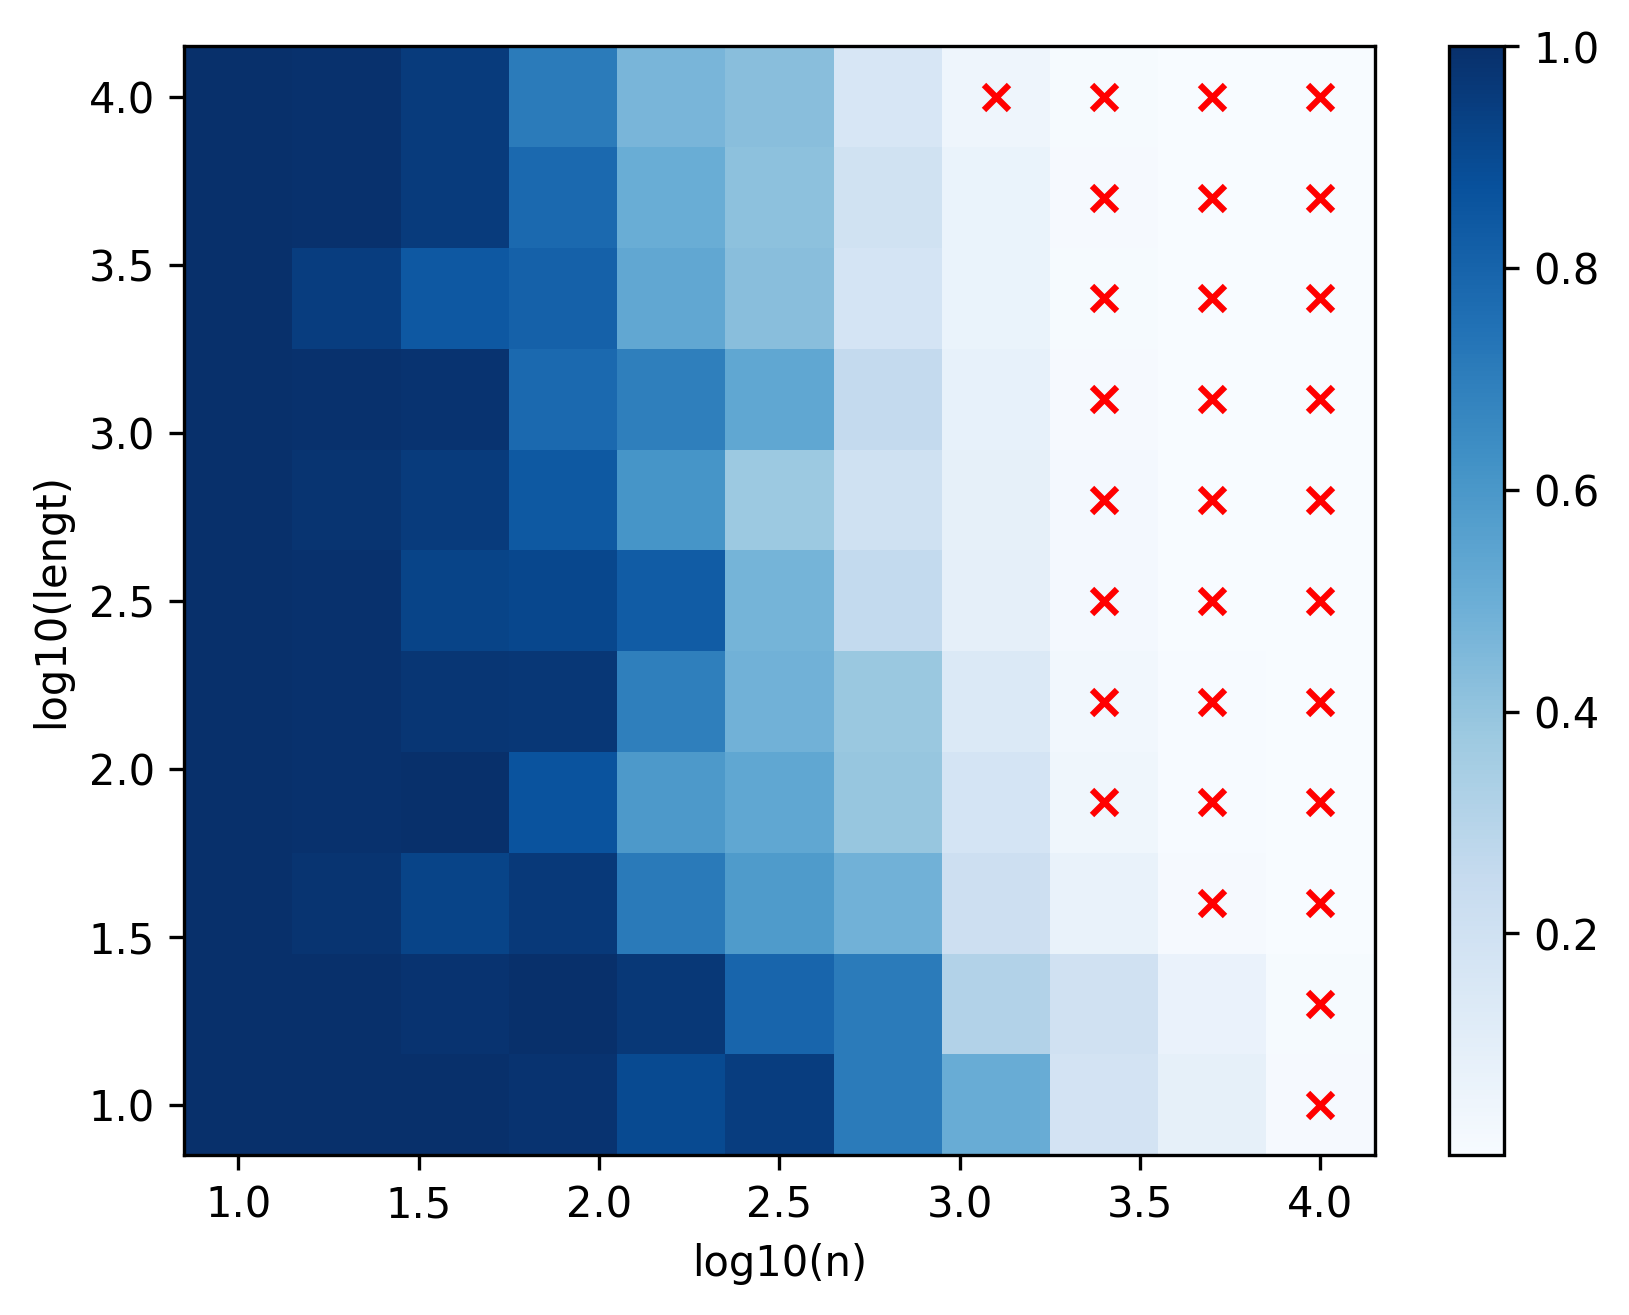
\includegraphics[width=0.6\textwidth]{figures/2samp-ssrw-af.png}
		\caption{2-sample test between Asymptotically Free SIRW and SSRW}
	\end{figure}
	\pause
	The test rejects null hypothesis, as expected.
\end{frame}

\begin{frame}
	\frametitle{Results of Adapted KS Test}
	\begin{figure}[htpb]
		\centering
		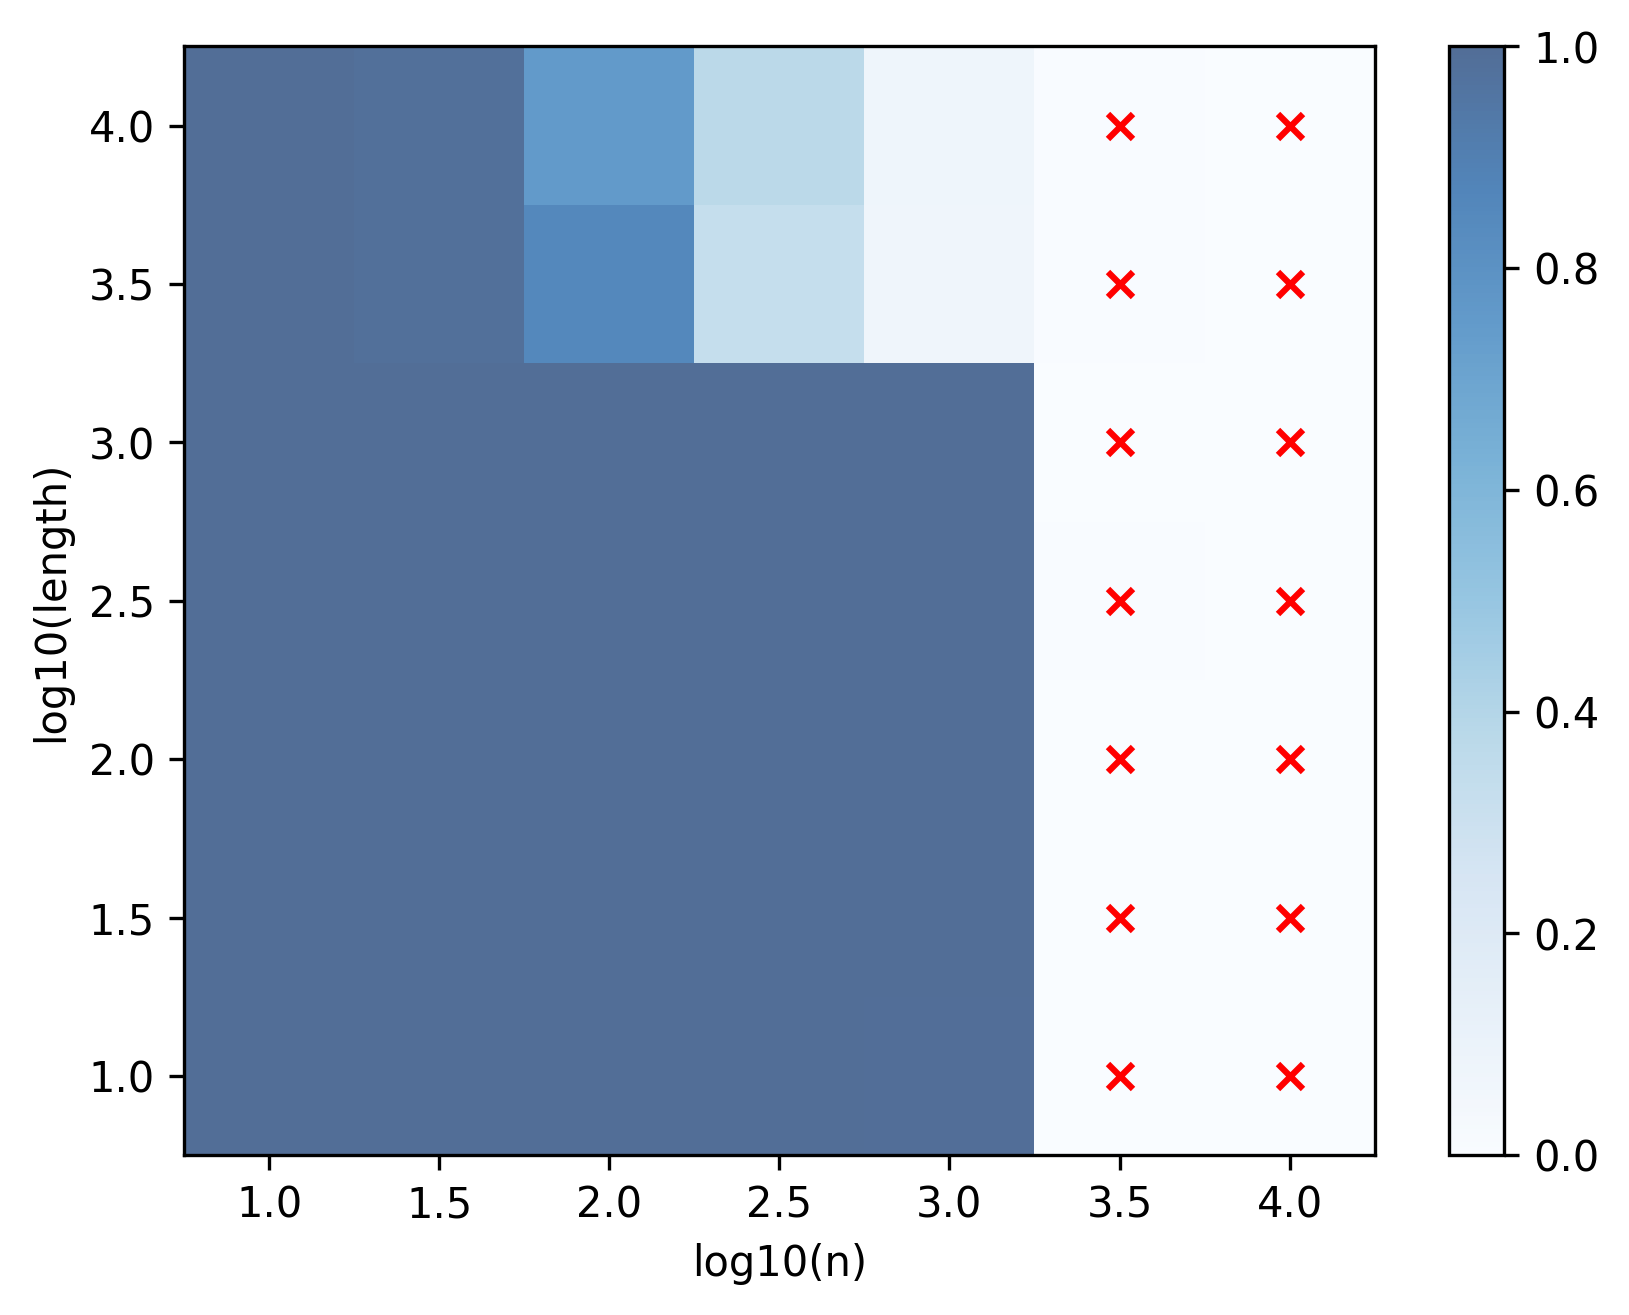
\includegraphics[width=0.6\textwidth]{figures/2samp-psr-bmpe.png}
		\caption{2-sample test between Polynomially Self-Repelling SIRW and BMPE}
	\end{figure}
	\pause
	The test rejects null hypothesis, as expected.
\end{frame}

\subsection*{Test on Time spent to the Right of Origin}

\begin{frame}
\frametitle{Fraction of Time to the Right of Origin}
	
Write $F^+_t(X_{\le t})$ to be the fraction of time spent to the right of origin
\[
	F^+_t(X_{\le t}) = \frac{1}{t} \int_0^t 1(X_s > 0) d s
.\] 


\cite{carmonaBetaVariablesTimes1998} shows that for $(X_t)_{t \in [0,1]} \sim \text{BMPE}(\alpha, \beta)$, $F^+(X) := F^+_1 (X_{\le 1})$ is distributed as $\text{Beta}\left( \frac{1-\alpha}{2}, \frac{1 - \beta}{2} \right) $.

\pause

{\color{blue}
This provides us a \textit{test statistic} for verifying if something is BMPE.}

\end{frame}

\begin{frame}
	Given the following theorem is true,
	\begin{theorem}
		If some random walk $(X_n)_{n \in \mathbb{N}}$ has a scaled limit of brownian motion perturbed at extrema:
\[
\left(\frac{X_{\lfloor n t\rfloor}}{\sqrt{n}}\right)_{t \in[0,1]} \Rightarrow(\alpha, \beta)\mathrm{-BMPE}
\]
then the fraction of time spent to the right of origin converges to a specific Beta distribution:
\[
F^+_n(X_{\le n}) = \frac{1}{n} \sum_{k=1}^n 1_{X_k>0} \Rightarrow \operatorname{Beta}\left(\frac{1-\alpha}{2}, \frac{1-\beta}{2}\right)
\]
	\end{theorem}
	we can directly test if $F^+(X_n)$ converge to corresponding beta distribution. If not, $X_n$ cannot converge BMPE under scaling.
\end{frame}

\begin{frame}
	\frametitle{Result of $F^+$ test}
	For fixed $w(n)$, We obtain an empirical distribution for $F^+_N$, $N = 10^4$, by generating  $10^3$ samples.
	\begin{figure}
\centering
\begin{minipage}{.5\textwidth}
  \centering
		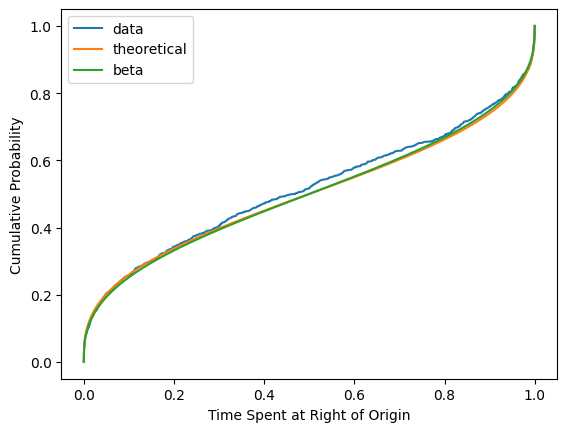
\includegraphics[width=0.8\textwidth]{figures/beta-fitting-af.png}
\end{minipage}%
\begin{minipage}{.5\textwidth}
  \centering
		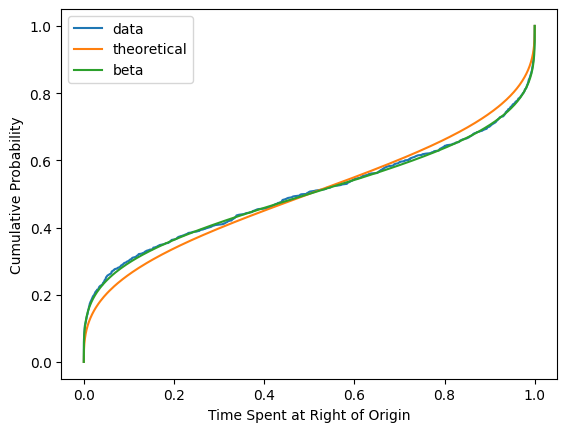
\includegraphics[width=0.8\textwidth]{figures/beta-fitting-psr.png}
\end{minipage}
\end{figure}
\pause

	Empirical distribution aligns well with $\text{Beta}(\gamma, \gamma)$ only for asymptotically free SIRW. 

\pause

	For polynomial self-repelling RW, empirical distribution differs significantly with $\text{Beta}(\gamma, \gamma)$. Nevertheless, we found no evidence showing it's not a beta distribution. 

\end{frame}

\section{Continuity Theorem}

\begin{frame}
	We now verify
\begin{theorem}
		If some random walk $(X_n)_{n \in \mathbb{N}}$ has a scaled limit of brownian motion perturbed at extrema:
\[
\left(\frac{X_{\lfloor n t\rfloor}}{\sqrt{n}}\right)_{t \in[0,1]} \Rightarrow(\alpha, \beta)\mathrm{-BMPE}
\]
then the fraction of time spent to the right of origin converges to a specific Beta distribution:
\[
F^+_n(X_{\le n}) = \frac{1}{n} \sum_{k=1}^n 1_{X_k>0} \Rightarrow \operatorname{Beta}\left(\frac{1-\alpha}{2}, \frac{1-\beta}{2}\right)
\]
	\end{theorem}
	\pause
	Suffices to verify that $F^+_{[0,1]}$ is continuous with respect to the Skorohod topology of cadlag functions on $[0,1]$.
\end{frame}

\begin{frame}
	It suffices to show
	\begin{lemma}
		For any $\varepsilon>0$, and almost every cadlag function $X_t$ on $[0,1]$, there exists $\delta>0$ such that whenever $d(Y_t, X_t) < \delta$, we have $|F^+(X_t) - F^+(Y_t)|< \varepsilon$.

		where $d$ is the Skorohod metric
		 \[
			d(x,y) := \inf _{\lambda \in \Lambda}\{\|\lambda-I\| \vee\|x-y \circ \lambda\|\}
		.\] 
	\end{lemma}
	\pause

	The problem: small vertical translation can drastically change $F^+(X_t)$, but $d$ is not sensitive to such vertical nudges. 
\begin{figure}[ht]
    \centering
    \incfig{vertical-nudge}
    \caption{vertical-nudge}
    \label{fig:vertical-nudge}
\end{figure}
	
\end{frame}

\begin{frame}
	\cite{kosyginaConvergenceNonconvergenceScaled2022} gives the cdf of $\text{BMPE}(\gamma, \gamma)$, which can be verified to be a continuous function. This is enough to show that the zero set of BMPE $X_t$ has measure zero almost surely.

	\pause

	Then we can cover the zero set with countably many open sets with total measure less than $\varepsilon$. Now consider the complement, which is compact and bounded some distance $r$ away from zero. 

	\pause

	By throwing out another set with total measure less than $\varepsilon$, we are end up with finitely many compact components, say there are $M$ components.

	\pause

	Then for $\delta< r$ small enough, it can be shown that for any $Y_t $ such that $d(X_t, Y_t) \le  r$,
	\[
		|F^+(X_t) - F^+(Y_t)| \le 2 M r + 2 \varepsilon
	.\] 
	which can be made arbitrarily small. QED.
\end{frame}



\section{Result Summary}

\begin{frame}
	\frametitle{A noticeable finding about PSR RW}

	Simulation shows that for PSR SIRW, the process stays entirely to the right of origin with positive probability.
\begin{figure}
\centering
\begin{minipage}{.5\textwidth}
  \centering
		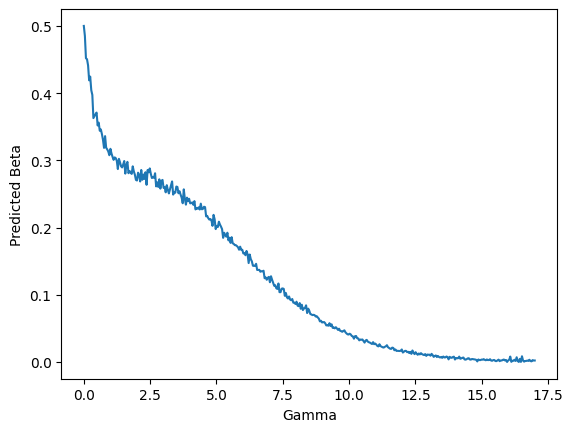
\includegraphics[width=0.8\textwidth]{figures/beta-fitting-gamma.png}
\end{minipage}%
\begin{minipage}{.5\textwidth}
  \centering
		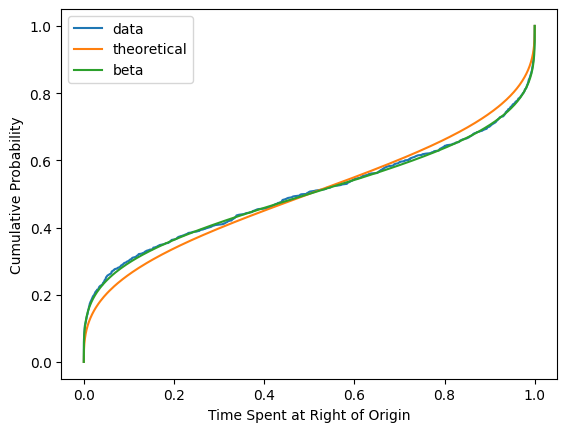
\includegraphics[width=0.8\textwidth]{figures/beta-fitting-psr.png}
\end{minipage}
\end{figure}

	
\end{frame}

\begin{frame}
	\frametitle{Summary of Results and Future Work}
	\begin{itemize}
		\item We developed statistical tools to probe limiting behavior of discrete random walks.
		\item<2-> The numerical methods we developed can be applied to provide empirical evidences to conjectures about limiting behavior of PSR random walks.
		\item<3-> Next step: Study the convergence of PSR random walk.
	\end{itemize}
\end{frame}



\begin{frame}
    \printbibliography
\end{frame}

\end{document}
